Huizenga et al. \citep{huizenga1995equivalent} show that scalp potential fields are contaminated by heteroscedastic noise in EEG measurements. We evaluate FANTOM’s performance in detecting epileptic regimes using EEG signals from 10 different patients in the Temple University Hospital EEG Seizure Corpus (TUSZ) dataset \citep{tang2021self}. The dataset encompasses multiple seizure types; in this study, we focus on generalized seizures, which engage the entire brain. Each patient’s record contains scalp EEG signals from 19 channels (Figure \ref{EEGsig}), each considered a causal variable.

\begin{figure}
    \centering
    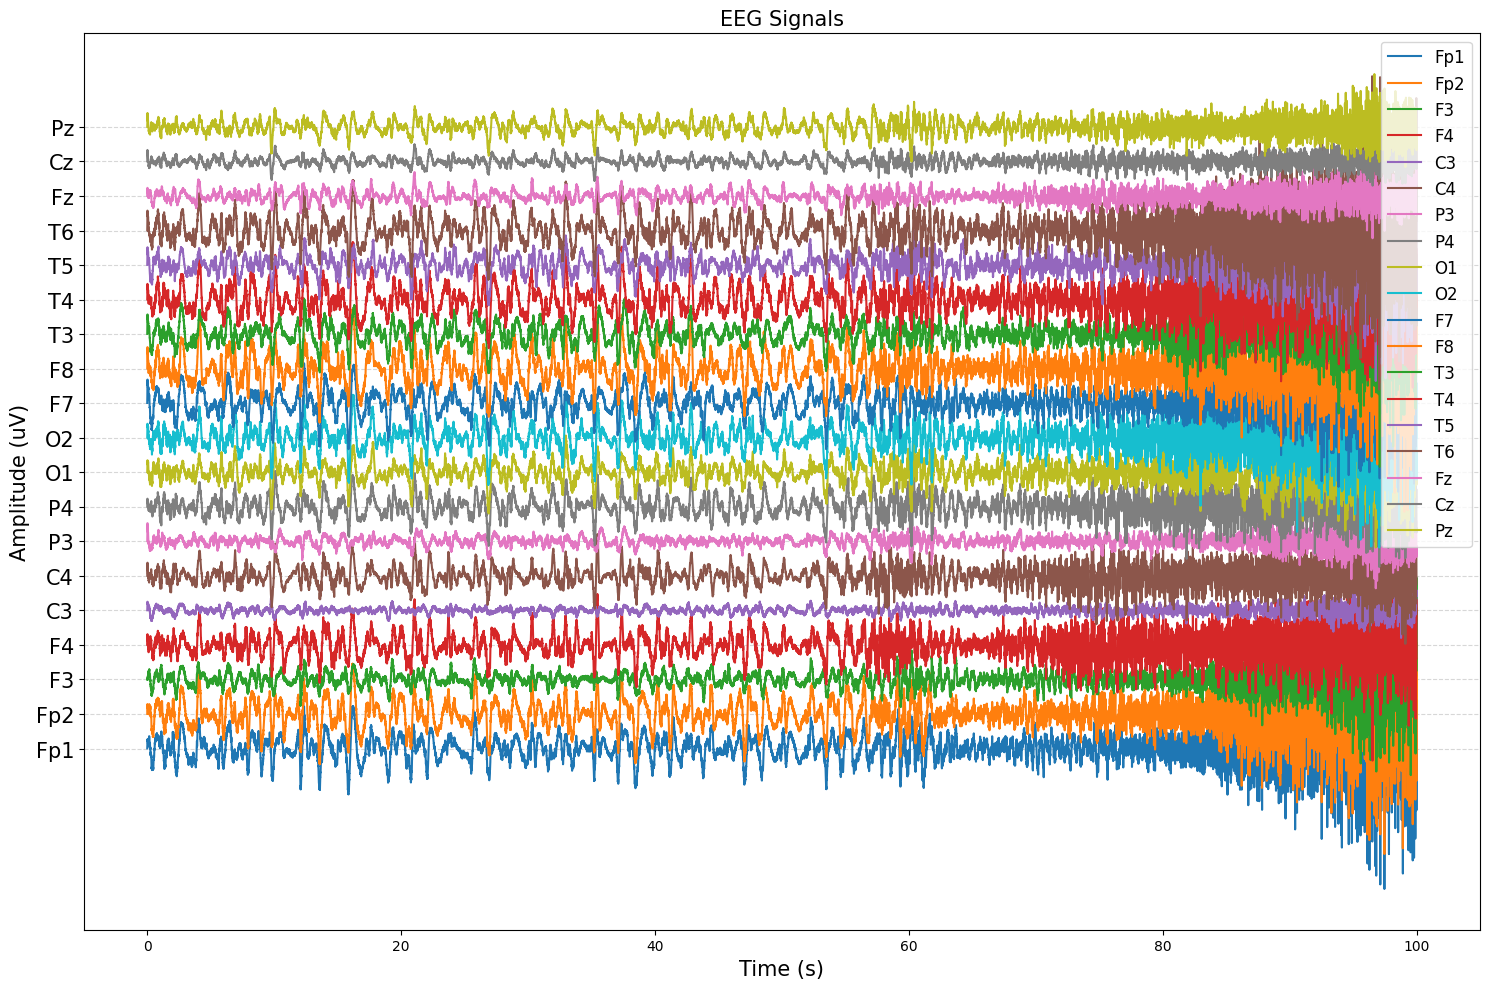
\includegraphics[width=0.8\linewidth]{figures/EEG_signal_7170.png}
    \caption{EEG signals for patient of id 7170, session 1 in the TUSZ data.}
    \label{EEGsig}
\end{figure}

State-of-the-art methods \citep{tang2021self} use graph neural networks (GNNs) for seizure detection, typically building a fixed distance graph and feeding Fast Fourier Transform (FFT) coefficients from 10–12 seconds EEG windows as node features. These approaches (i) train a single model for all patients, offering no personalization; (ii) cannot operate in zero-shot or unsupervised settings; and (iii) reuse an identical graph for both seizure and normal periods. FANTOM addresses these limitations: it detects seizures in a personalized manner without any training data and learns distinct temporal causal graphs for normal and seizure states. 

\textbf{Preprocessing. }We apply FANTOM to 10 different patients from TUSZ dataset, we treat this as an unsupervised regime detection problem, analyzing roughly 100 seconds of recordings at a 250 Hz sampling rate for each patient, capturing both normal and seizure states. Before running FANTOM, we filter out the EEG signals by a band pass filter of order 6, the lower frequency is 0.5Hz while the highest frequency is 50Hz.

\begin{table}[H]
\centering
\caption{Seizure detection accuracy using FANTOM for 10 different patients}   
\begin{tabular}{@{}c|c@{}}
\toprule
Patient id & Regime Acc \\ \midrule
0002       & 84.8       \\
0021       & 80.8       \\
0302       & 76.6       \\
0492       & 86.6       \\
6440       & 86.1       \\
6520       & 80.2       \\
7128       & 94.1       \\
7170       & 81.1       \\
7936       & 82.0       \\
8303       & 75.1       \\ \midrule
Avg       & $82.7_{\pm 5.2}$\\ \bottomrule
\end{tabular}
\label{EEG_table}
\end{table}
We segment each EEG recording into fixed 12 s windows (3000 samples). FANTOM is initialized with eight initial regimes and reliably converges to the two ground-truth states; quantitative results appear in Table \ref{EEG_table}. We employ a temporal lag of eight samples and allow instantaneous parental links. Averaged over all patients, FANTOM achieves 82.7\% regime-assignment accuracy. The graph learned for the seizure state is substantially denser and more interconnected than that of the normal state (Figure \ref{EEG_graphs}), consistent with the widespread neural involvement of generalized seizures. 
\begin{figure}
    \centering
    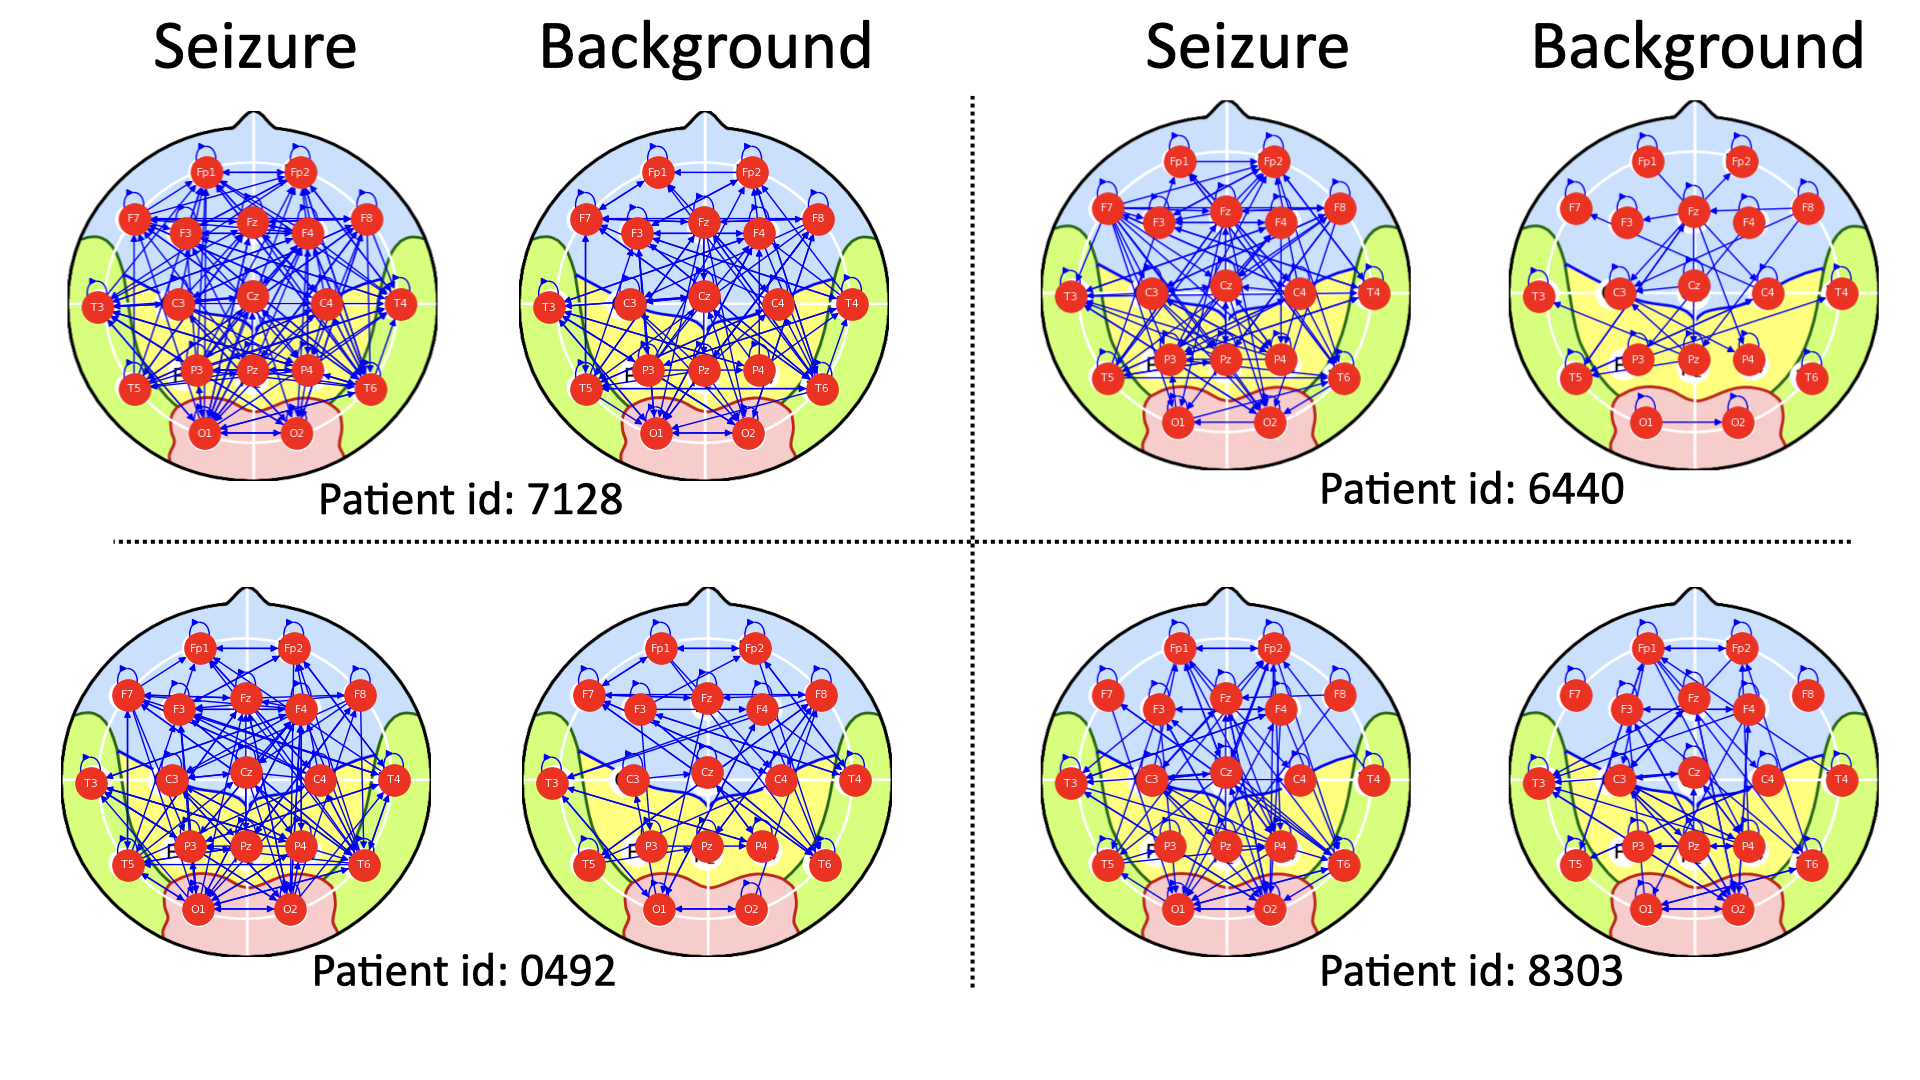
\includegraphics[width=1\linewidth]{figures/sz_bg_epilepsy_fantom_results.001.png}
    \caption{Figure illustrates the summary causal graph per regime learned by FANTOM for different patients}
    \label{EEG_graphs}
\end{figure}